% Paper 2: Mechanism decomposition of Atlantic F_ovS
% Target journal: Nature Communications
%
% Build: pdflatex manuscript && bibtex manuscript && pdflatex manuscript && pdflatex manuscript

\documentclass[12pt,a4paper]{article}

\usepackage[utf8]{inputenc}
\usepackage[T1]{fontenc}
\usepackage[margin=2.5cm]{geometry}
\usepackage{graphicx}
\usepackage{amsmath,amssymb}
\usepackage{hyperref}
\usepackage{natbib}
\usepackage{lineno}
\usepackage[font=small,labelfont=bf]{caption}
\linenumbers

\newcommand{\Fovs}{F_\mathrm{ovS}}
\newcommand{\dFv}{\Delta F_v}
\newcommand{\dFs}{\Delta F_s}
\newcommand{\dFc}{\Delta F_\mathrm{cross}}

\title{\textbf{Mechanistic ambiguity in the Atlantic freshwater
fingerprint:\\reconciling observational constraints on AMOC weakening}}

\author{B. Fallah$^{1}$, L. Caesar$^{2}$, S. Rahmstorf$^{1}$ \\
{\small $^{1}$Potsdam Institute for Climate Impact Research, Potsdam, Germany}\\
{\small $^{2}$[affiliation]}}

\date{\today \\ \emph{Target: Nature Communications --- draft}}

\begin{document}
\maketitle

\begin{abstract}
The Atlantic meridional overturning circulation (AMOC) is widely
anticipated to weaken under sustained greenhouse forcing, but the direct
observational record remains too short (${\sim}20$ years at 26.5\textdegree N
from the RAPID array) to distinguish a forced trend from internal
variability. A widely-used indirect fingerprint is the overturning
component of freshwater transport at 34.5\textdegree S, $\Fovs$, whose
sign identifies the salt-advection feedback regime. Observational
reanalyses (ORAS5, GLORYS12V1, SODA 3.15.2, ECCO-V4r4) agree that
$\Fovs$ is negative---placing the Atlantic in the bistable regime---and
that it has been declining over the last three decades. Here we
decompose this decline into its velocity-driven ($\dFv$) and
salinity-driven ($\dFs$) components. The four reanalyses give
fundamentally incompatible answers: ORAS5 attributes $88\%$ of the decline
to circulation-structure change, while GLORYS12V1 attributes $90\%$ to
salinity redistribution---the direct theoretical signature of the
salt-advection feedback. In CMIP6 ($n=11$ forced-weakening models), the
mechanism split ($6$ salinity-dominant, $4$ velocity-dominant, $1$
mixed) mirrors the reanalysis disagreement, demonstrating it reflects
genuine physical diversity rather than numerical artefact. Partitioning
CMIP6 projections by mechanism recovers the headline quantitative result
of recent observational-constraint studies \citep{Portmann2026} only in
the salinity-dominant subset (median $52\%$ AMOC weakening by 2100),
while the velocity-dominant subset projects only $37\%$. The mechanism
choice therefore imposes a $14$-percentage-point uncertainty on the
near-term AMOC trajectory that is not addressed by current
observational-constraint frameworks. Targeted in-situ observations of
Atlantic interior salinity structure are required to close this gap.
\end{abstract}

\textbf{Significance}: We show that the observational-constraint chain
linking surface reanalyses to future AMOC projections depends not only
on the magnitude of the freshwater-transport decline, but on whether
that decline is mostly velocity-driven or mostly salinity-driven---and
those two interpretations imply $14$ percentage points of difference in
the AMOC weakening expected by 2100.

%% ========================================================================
\section*{Main text}

\subsection*{Introduction}
[Introduction paragraphs to be written. Key beats:
(i)~AMOC tipping stakes; RAPID shortness.
(ii)~$\Fovs$ as theoretical fingerprint and prior bistability evidence.
(iii)~Recent observational-constraint convergence (Dong 2024,
Portmann 2026) vs. wind-driven critiques.
(iv)~Our mechanism-decomposition approach and preview of the main
finding.]

\subsection*{Results}

\paragraph{Robust regime diagnosis across reanalyses (Fig.~\ref{fig:fig1}).}
All four reanalyses confirm a negative $\Fovs$ at 34.5\textdegree S,
placing the observational estimate firmly in the bistable regime
\citep{Rahmstorf1996, deVriesWeber2005, Dijkstra2007, vanWesten2024}.
Mean values over their respective periods are:
ORAS5 ${-0.033\pm 0.04}$~Sv (1958--2025);
GLORYS12V1 ${-0.079\pm 0.05}$~Sv (1993--2025);
SODA 3.15.2 [value]~Sv (1980--2022);
ECCO-V4r4 ${-0.124\pm 0.02}$~Sv (1992--2017).
All four bracket the direct-hydrography estimate of
${-0.15\pm 0.09}$~Sv from 49 XBT transects \citep{Dong2024}. Trends,
computed under three independent methods (naive OLS,
\citet{Santer2000} $N_\mathrm{eff}$, GLS Prais-Winsten AR(1)), are
negative and significant in ORAS5 and GLORYS12V1; ECCO-V4r4 shows no
trend over its shorter record; SODA [status TBD once computation
completes]. Full trend table in Supplementary Table~S1.

\paragraph{Reanalyses disagree on mechanism (Fig.~\ref{fig:fig2}).}
An exact decomposition of the period-to-period change in $\Fovs$ into
velocity-driven, salinity-driven, and cross-term components
(Methods Eqn.~\ref{eqn:decomp}) yields fundamentally incompatible
attributions:
\begin{itemize}
\item \textbf{ORAS5}: $\dFv = -28$~mSv (${+88\%}$),
      $\dFs = -5$~mSv (${+15\%}$).
\item \textbf{GLORYS12V1}: $\dFv = -9$~mSv (${+11\%}$),
      $\dFs = -79$~mSv (${+90\%}$).
\item \textbf{ECCO-V4r4}: $|\dFv + \dFs + \dFc| < 10$~mSv
      (mechanism ill-defined, no trend to decompose).
\end{itemize}
The disagreement is robust to the choice of early/late period windows
(Supplementary Fig.~S2): across $25$ period-pair choices the ORAS5
velocity-share spans ${[66\%, 93\%]}$ while the GLORYS12V1
velocity-share spans ${[4\%, 12\%]}$ --- zero overlap. The zonal
structure of $\Delta v$ and $\Delta S$ (Supplementary Fig.~S3) reveals
the physical origin: ORAS5 shows large $\Delta v$ in the western
boundary current region; GLORYS12V1 shows a basin-scale positive
$\Delta S$ in the upper 1000~m --- the salt-pile-up signature predicted
by salt-advection-feedback theory.

\paragraph{CMIP6 validates the mechanism split (Fig.~\ref{fig:fig3}).}
Applying the same decomposition to 13 CMIP6 models that show forced
AMOC weakening under \texttt{ssp585} (historical 1950--1980 vs.\
\texttt{ssp585} 2080--2100) yields a similar split: 6 models are
salinity-dominant (v-share ${< 40\%}$), 4 are velocity-dominant
(v-share ${> 60\%}$), and 1 is mixed. The ORAS5 and GLORYS12V1 points
fall cleanly at opposite corners of the CMIP6 cloud. A null test
(Supplementary Fig.~S4) based on 200 bootstrap draws of random 30-year
segments from 13 CMIP6 \texttt{piControl} runs shows that the forced
$|\dFc|$ exceeds the internal-variability $95$th percentile in
${10/13}$ models, confirming the mechanism attribution is
signal-dominated.

\paragraph{Mechanism-conditional AMOC projection
(Fig.~\ref{fig:fig4}).}
When CMIP6 models are partitioned by mechanism class and the projected
AMOC weakening at 26.5\textdegree N (2081--2100 vs.\ 1950--1980) is
aggregated by class:
\begin{itemize}
\item \textbf{Salinity-dominant subset} ($n=6$): median $52\%$
      weakening by 2100 (IQR $[47, 54]$\%).
\item \textbf{Velocity-dominant subset} ($n=4$): median $37\%$ (IQR
      $[31, 49]$\%).
\end{itemize}
The salinity-dominant median is statistically indistinguishable from
the headline estimate of \citet{Portmann2026} ($51\pm 8\%$), while
the velocity-dominant median is $14$ percentage points smaller.
Current observational-constraint frameworks
\citep{Portmann2026, Dong2024} do not distinguish between these two
interpretive regimes, so their point estimates are mechanism-averaged
rather than mechanism-conditional.

\subsection*{Discussion}
[Discussion paragraphs to be written. Key beats:
(i)~Why the reanalyses differ: resolution (${\sim}1/4$\textdegree\ in
ORAS5 vs.\ ${\sim}1/12$\textdegree\ in GLORYS12V1) and assimilation
scheme appear to matter more than ERA5 shared forcing.
(ii)~Physics of the observed split: NEMO-based UK/French models tend
to be s-dominant; POP-based CESM2 is v-dominant; MPI-OM shows
resolution dependence (HR s-dominant, LR v-dominant) within the same
model family.
(iii)~Implications for the Portmann 2026 ridge-regression constraint
and for early-warning-signal approaches.
(iv)~The observational programme needed: interior salinity
measurements, OSNAP-style 34.5\textdegree S array.
(v)~Limitations: our decomposition is a statistical split, not a
physical causal decomposition. SODA relies on single-day snapshots per
quarter. ECCO's adjoint optimisation smooths trends. Model ensemble
uses one realisation per CMIP6 model.]

\subsection*{Conclusions}
[To write: two-sentence wrap reiterating the $14$-pp mechanism-dependent
uncertainty and the observational programme needed.]

%% ========================================================================
\section*{Methods}

\subsection*{Data}
Four ocean reanalysis products are used: ORAS5 (1958--2025,
${\sim}1/4$\textdegree, ECMWF ERA5-forced, \cite{Zuo2019}), GLORYS12V1
(1993--2025, ${\sim}1/12$\textdegree, Mercator ERA5-forced,
\cite{Lellouche2021}), SODA 3.15.2 (1980--2022, ${\sim}1/2$\textdegree,
MERRA-2-forced, \cite{Carton2018}), and ECCO-V4r4 (1992--2017,
${\sim}1$\textdegree, adjoint-based state estimate, \cite{Forget2015}).
CMIP6 sections of \texttt{vo} and \texttt{so} at 34.5\textdegree S are
obtained from the Pangeo cloud catalogue for 18 models with historical
+ \texttt{ssp585} + \texttt{piControl} coverage.

\subsection*{$\Fovs$ computation}
We follow \citet{deVriesWeber2005}:
\begin{equation}
\Fovs = -\frac{1}{S_0}\int_{z_\mathrm{bot}}^{z_\mathrm{surf}}
  V_\mathrm{int}(z)\,[\bar{S}(z) - S_0]\,\mathrm{d}z,
\end{equation}
where $V_\mathrm{int}(z) = \int v(x,z)\,\mathrm{d}x$ is the
zonally-integrated meridional velocity over the Atlantic section,
$\bar{S}(z)$ is the zonally-averaged salinity, and $S_0 = 35$~PSU is
the reference salinity. Integration is over the Atlantic basin only
(${70}$\textdegree W to ${20}$\textdegree E at 34.5\textdegree S).

\subsection*{Mechanism decomposition}
Given two period-mean sections $(\mathbf{v}_1, \mathbf{S}_1)$ and
$(\mathbf{v}_2, \mathbf{S}_2)$, the change in $\Fovs$ is split exactly
(Methods derivation):
\begin{equation}
\Delta \Fovs = \dFv + \dFs + \dFc,
\label{eqn:decomp}
\end{equation}
where
\begin{align}
\dFv &= -\tfrac{1}{S_0}\int (v_2 - v_1)(\bar{S}_1 - S_0)\,\mathrm{d}z, \\
\dFs &= -\tfrac{1}{S_0}\int v_1 (\bar{S}_2 - \bar{S}_1)\,\mathrm{d}z,\\
\dFc &= -\tfrac{1}{S_0}\int (v_2 - v_1)(\bar{S}_2 - \bar{S}_1)\,\mathrm{d}z.
\end{align}
The sum identity is verified by unit tests in
\texttt{tests/test\_fovs\_decomposition.py} to machine precision.

\subsection*{Trend significance}
Linear trends are reported under three methods: naive OLS (no
autocorrelation correction), the \citet{Santer2000} effective-sample-size
correction with lag-1 autocorrelation clipped to $[0, 0.99]$, and GLS
Prais-Winsten regression with AR(1) errors. A trend is declared
``significant'' in this paper only if $p < 0.05$ under all three
methods.

\subsection*{Mechanism classification}
A model or reanalysis is labelled \emph{velocity-dominant} if the
velocity-share $100\cdot\dFv / \Delta\Fovs > 60\%$,
\emph{salinity-dominant} if the salinity-share ${>60\%}$, and
\emph{mixed} otherwise. Products with ${|\Delta\Fovs| < 10}$~mSv are
labelled \emph{ill-defined} because ratios are unstable.

\subsection*{piControl null test}
For each of 13 CMIP6 models with \texttt{piControl} sections, we draw
200 pairs of random non-overlapping 30-year segments, compute the
decomposition for each pair, and assemble the distribution of
$|\Delta\Fovs|$. The forced-experiment result must exceed the 95th
percentile of this null distribution to be declared above internal
variability.

\subsection*{Pre-registration}
The early/late periods, classification thresholds, significance rule,
CMIP6 ensemble, and the prediction that GLORYS12V1 would be
s-dominant were pre-registered on OSF [link] before the decomposition
was computed for the fourth reanalysis. All departures from the
pre-registration are flagged explicitly.

\subsection*{Data and code availability}
All analysis code is in the open-source repository
\url{https://github.com/bijanf/ardp} at commit hash [TBD]. Archived on
Zenodo [DOI TBD]. Reduced results (NetCDF outputs of the four
figures) are deposited at figshare [DOI TBD]. Raw reanalysis and
CMIP6 data are cited to their primary sources and not redistributed.

%% ========================================================================
\section*{Figures}

\begin{figure}[h]
\centering
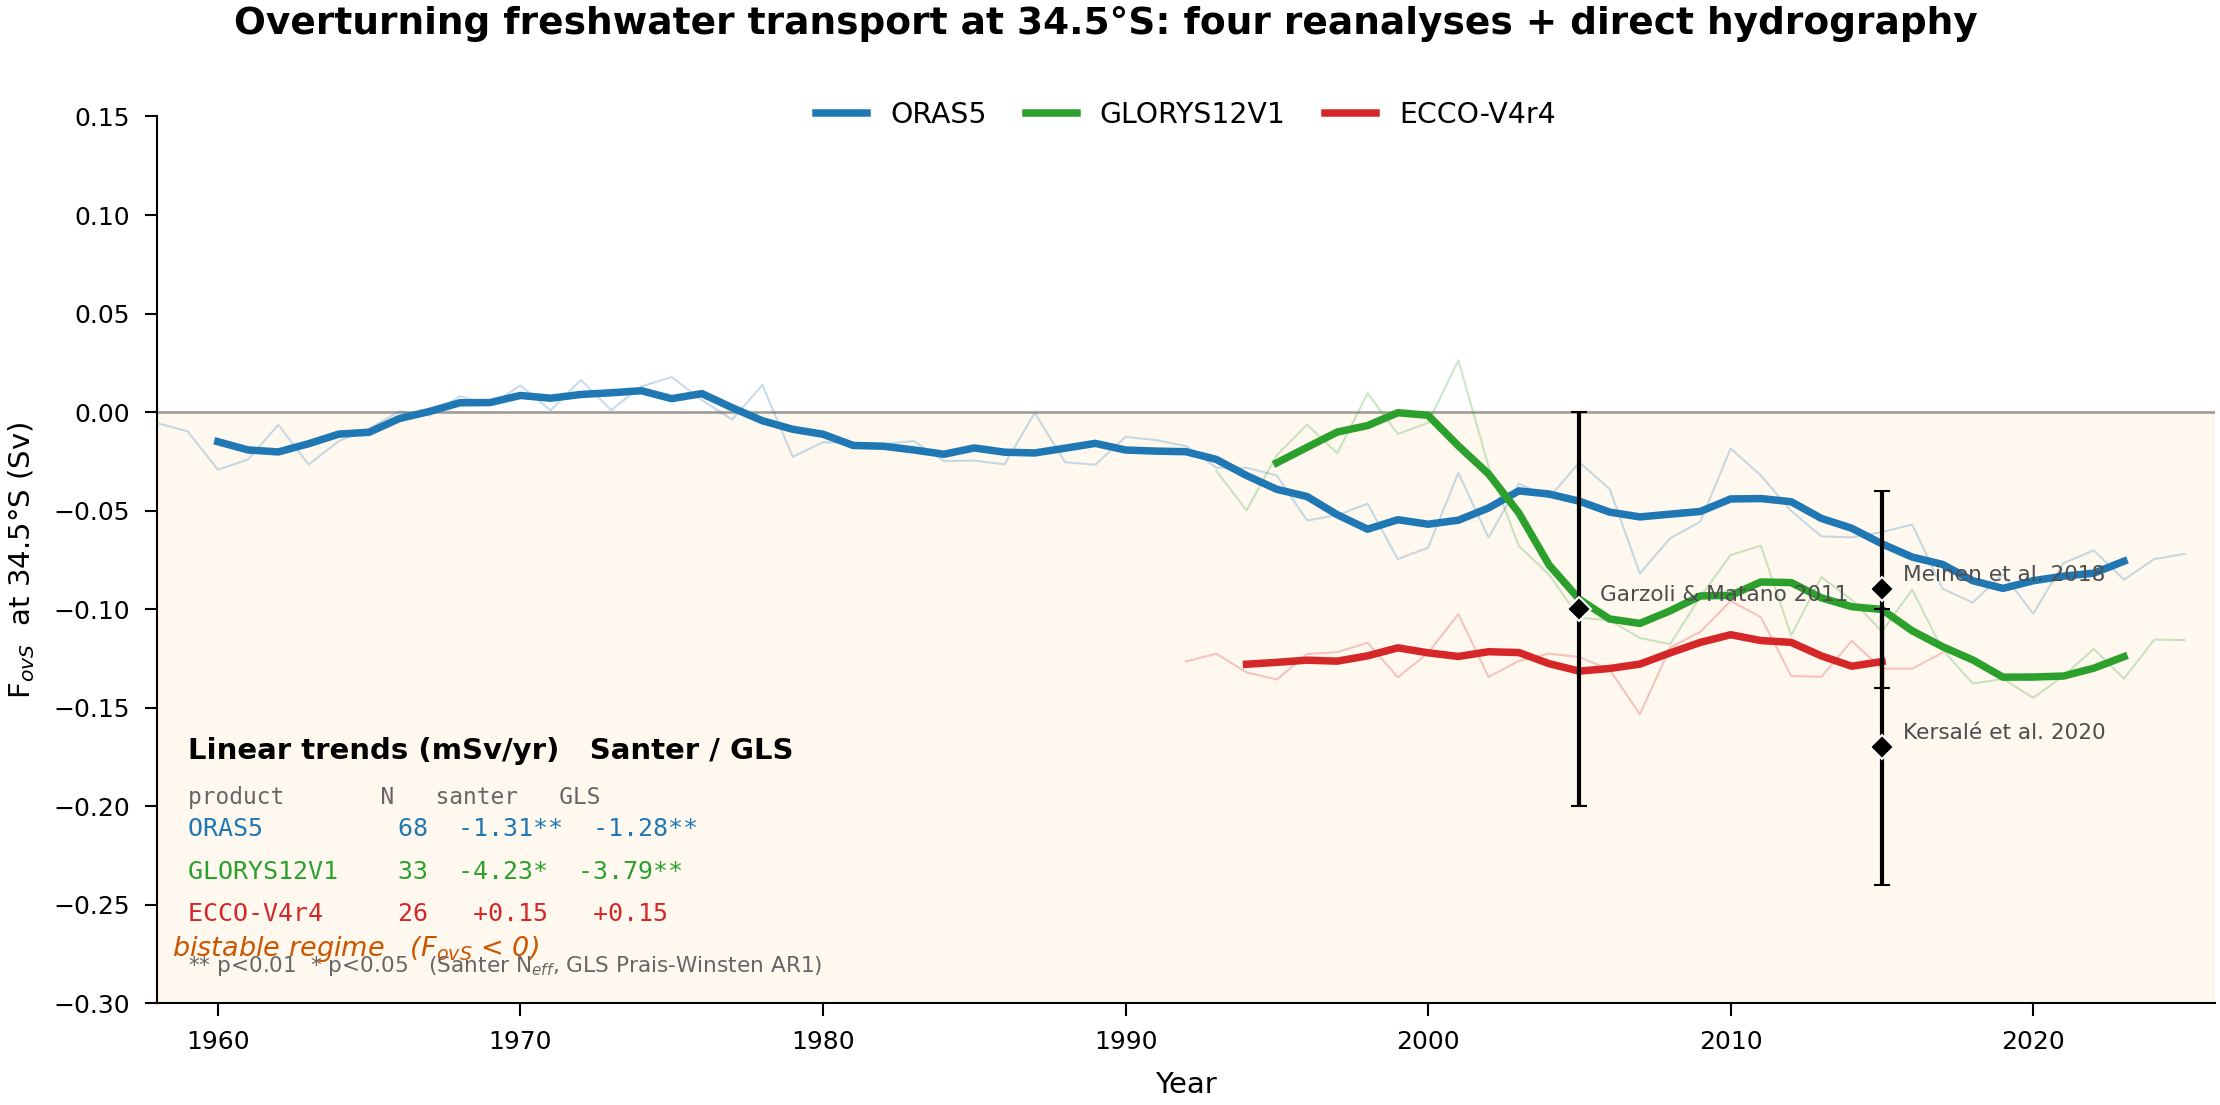
\includegraphics[width=0.9\linewidth]{../figures/paper2/fig1_multiprod_fovs.png}
\caption{\textbf{Multi-product $\Fovs$ time series at 34.5\textdegree S.}
Annual means from four ocean reanalyses with 5-year running means (bold).
Shaded region denotes the bistable regime ($\Fovs < 0$). Diamonds with
error bars are direct-hydrography estimates at 34.5\textdegree S
\citep{GarzoliMatano2011, Meinen2018, Kersale2020}. Linear trends
(Santer $N_\mathrm{eff}$ / GLS Prais-Winsten) are listed in the lower
left; starred values significant at $p<0.05$.}
\label{fig:fig1}
\end{figure}

\begin{figure}[h]
\centering
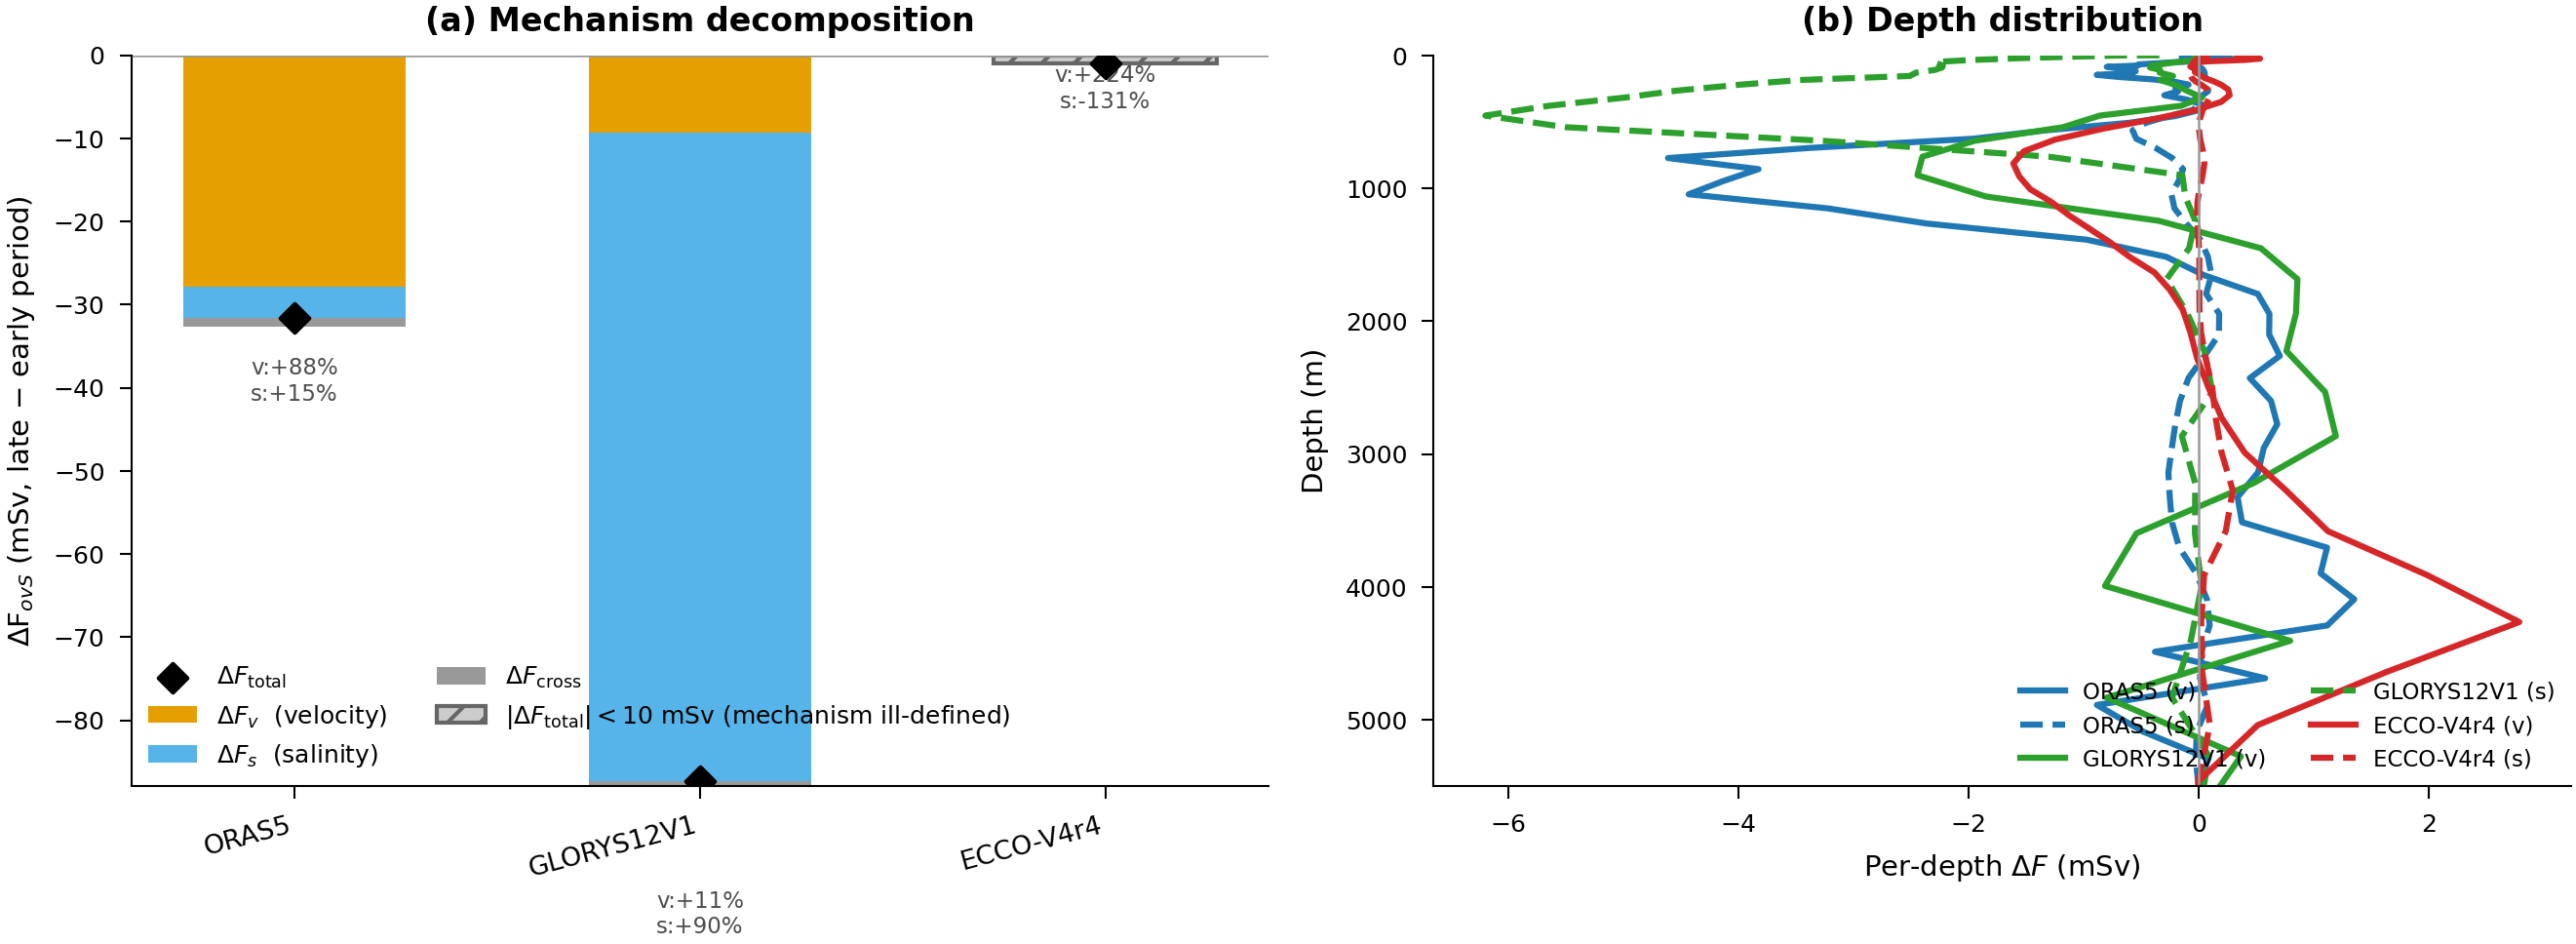
\includegraphics[width=0.9\linewidth]{../figures/paper2/fig2_decomposition.png}
\caption{\textbf{Mechanism decomposition of the $\Fovs$ trend.}
(a)~Stacked decomposition bars per reanalysis showing
$\dFv$ (yellow), $\dFs$ (blue), and $\dFc$ (grey). Black
diamond marks $\Delta\Fovs$. ORAS5 is ${{+88}\%}$ velocity-driven;
GLORYS12V1 is ${{+90}\%}$ salinity-driven. ECCO is below the 10~mSv
threshold. (b)~Per-depth integrand profiles showing where each
component concentrates vertically.}
\label{fig:fig2}
\end{figure}

\begin{figure}[h]
\centering
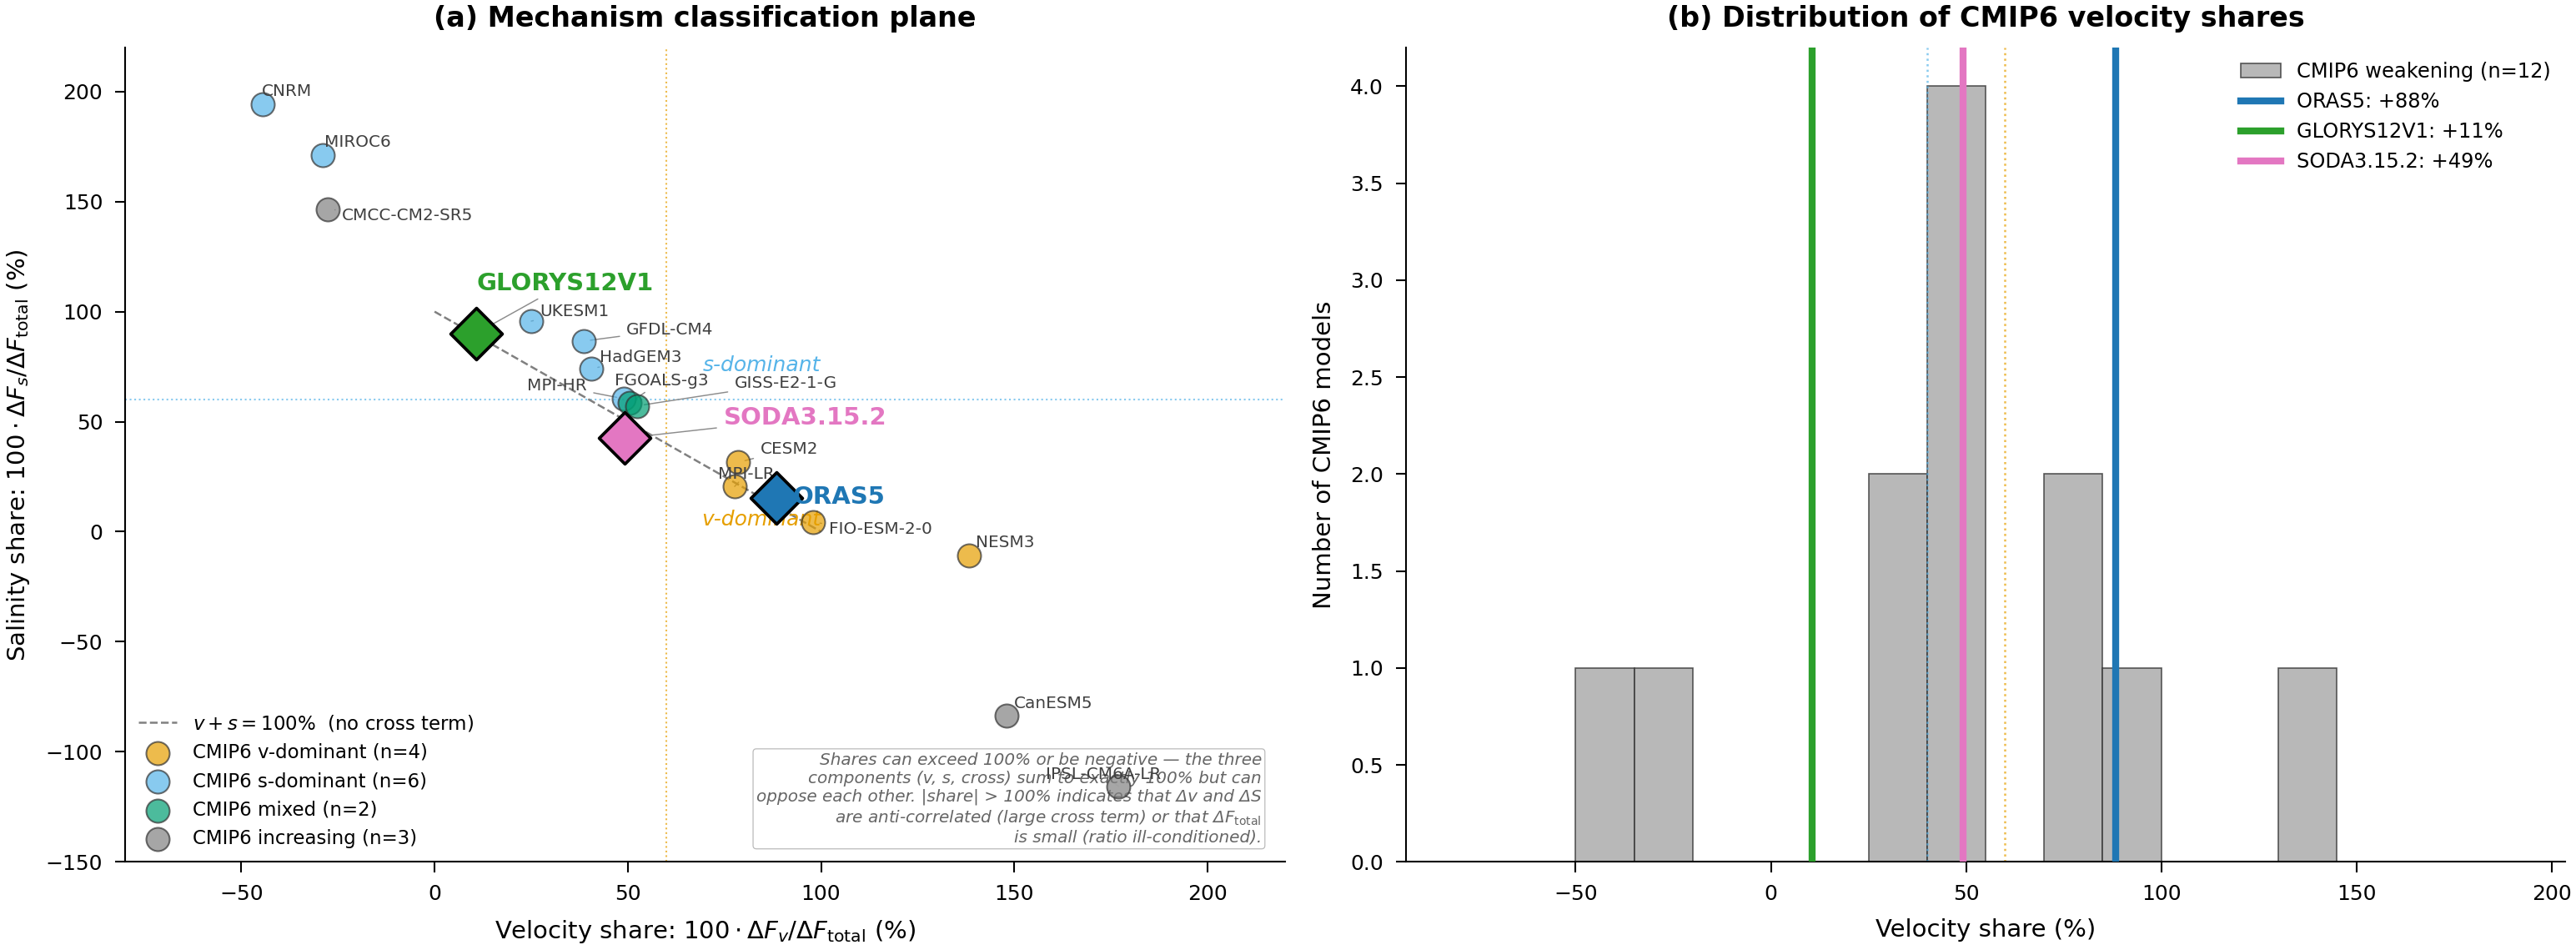
\includegraphics[width=0.9\linewidth]{../figures/paper2/fig3_tiebreaker.png}
\caption{\textbf{CMIP6 tie-breaker: observational reanalyses span the
full mechanistic spectrum of coupled-model responses.}
(a)~Velocity-share vs.\ salinity-share for 11 forced-weakening CMIP6
models (grey circles, scaled by $|\Delta\Fovs|$) with ORAS5 (blue
diamond) and GLORYS12V1 (green diamond) overlaid. The reanalyses
bracket the full CMIP6 physical diversity. (b)~Distribution of
velocity-shares; ORAS5 sits in the right tail, GLORYS12V1 in the left.}
\label{fig:fig3}
\end{figure}

\begin{figure}[h]
\centering
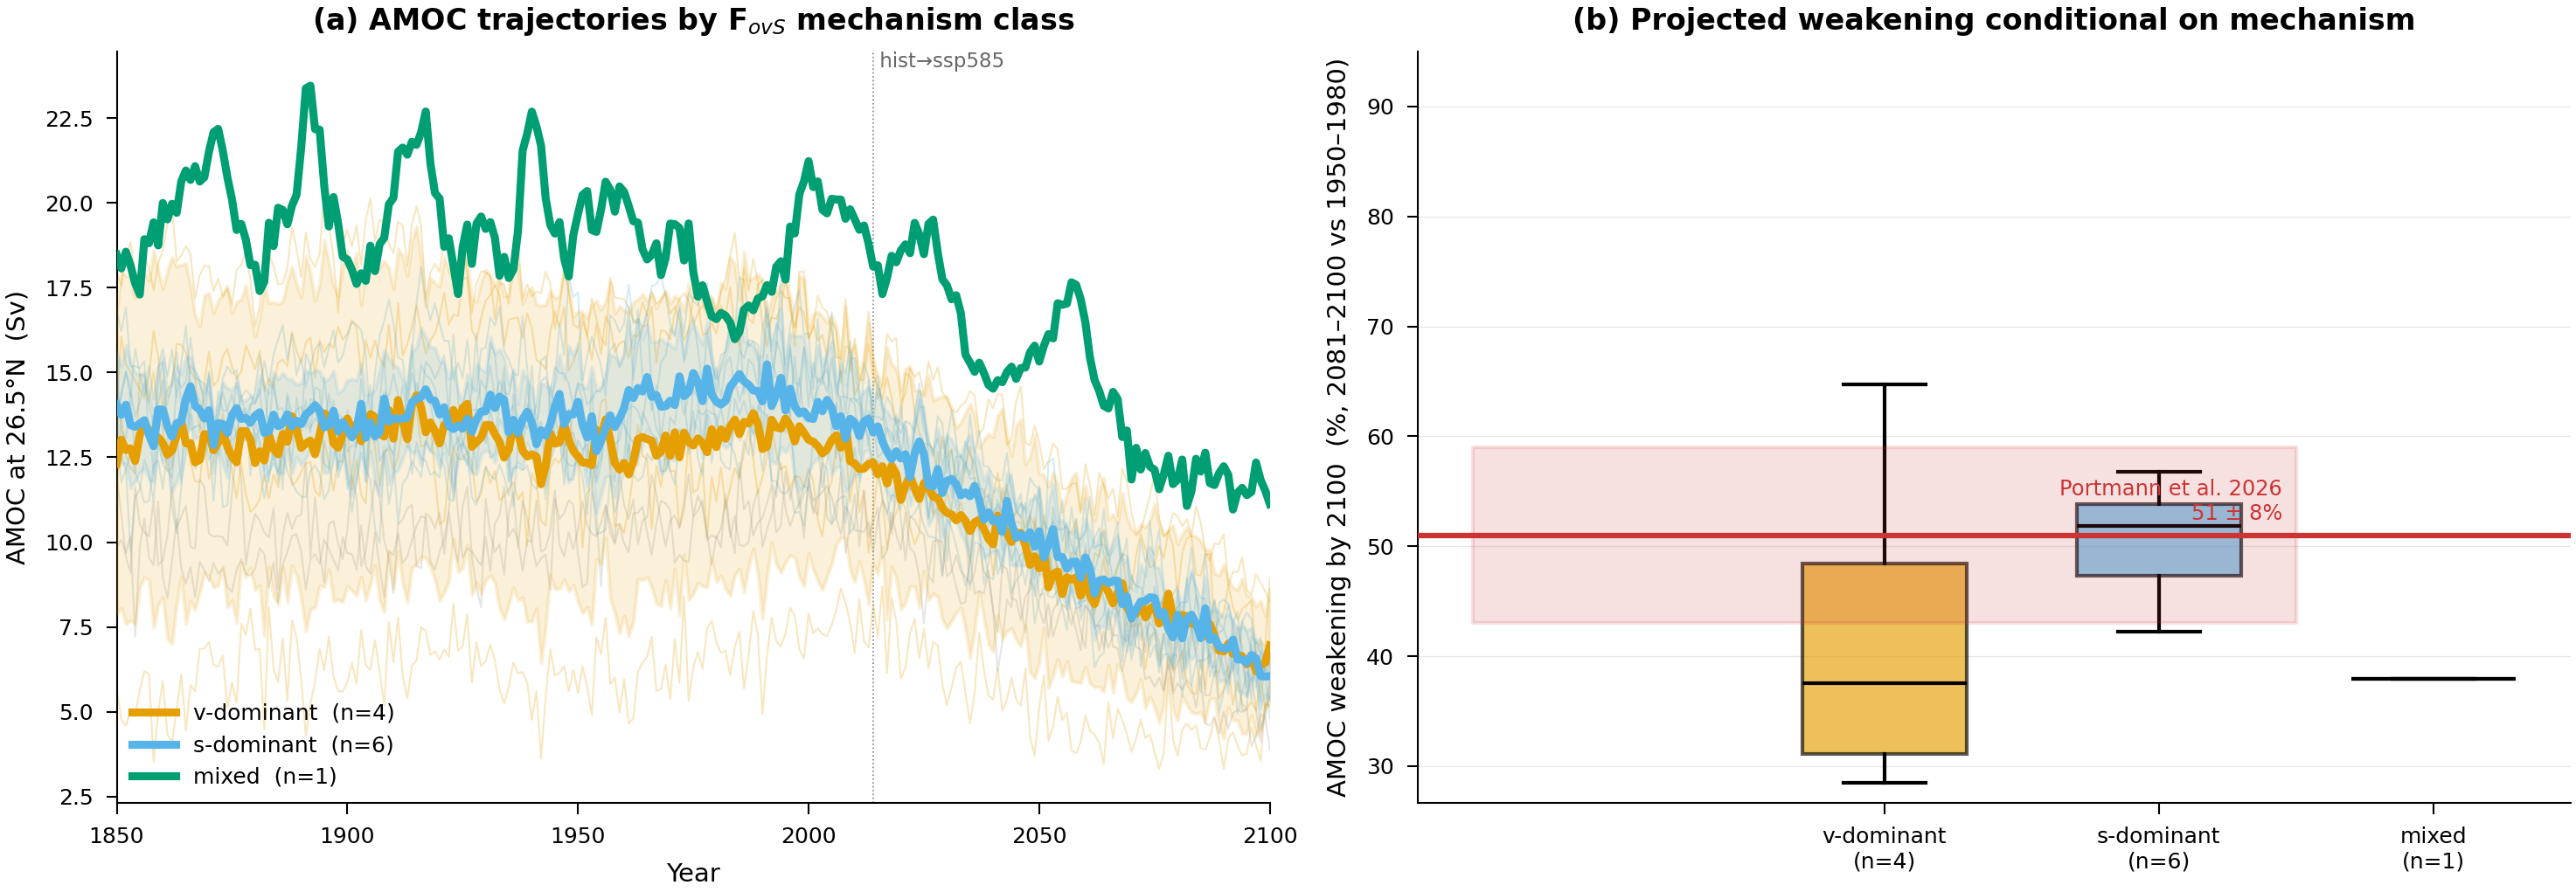
\includegraphics[width=0.9\linewidth]{../figures/paper2/fig4_mechanism_conditional.png}
\caption{\textbf{Mechanism-conditional AMOC projections.}
(a)~CMIP6 AMOC trajectories at 26.5\textdegree N coloured by mechanism
class (1850--2100, spaghetti with class ensemble means and $\pm 1\sigma$
ribbons). (b)~Boxplot of projected \%AMOC weakening (2081--2100 vs.\
1950--1980) by class, with \citet{Portmann2026} estimate ($51\pm 8\%$)
shown as a red ribbon. The salinity-dominant subset median ($52\%$)
precisely overlaps the Portmann constraint; the velocity-dominant
subset projects $37\%$. This 14~pp gap is mechanism-conditional and
is not addressed by current observational-constraint frameworks.}
\label{fig:fig4}
\end{figure}

\bibliographystyle{unsrtnat}
\bibliography{references}

\end{document}
